\chapter{Actores}

En este capitulo se explicara de como funciona la estructura computacional en modelo de actores. En la primera sección explicaran como funcionan las comunicaciones y el comportamiento de los actores. En la segunda se daran conceptos básicos para definir un lenguaje minimo de actores.

\section{Definiendo un Sistema de Actores}

Los calculos en un sistema de actores es en respuesta a las comunicaciones enviadas al sistema. Estas comunicaciones están representadas como \textit{tareas}. El sistema de actores evoluciona a partir de estas tareas, cuando una tarea es procesada genera nuevas tareas y nuevos actores. Todas las tareas que fueron proceadas y todos los actores que ya no son útiles pueden ser liberadas con algún tipo de ``Garabage Collector''. La idea de cuando un actor deja de ser útil será definida con mejor presición más adelante. Esto no afecta el comportamiento del sistema. La configuración de un sistema de actores viene dada por los actores que tiene, y el conjunto de tareas no proceadas.

\subsection{Tareas}

Podríamos decir que las \textit{tareas} que no son fueron procesadas son quienes mueven los calculos en un sistema de actores.

Las \textit{tareas} estan respresentadas por 2-tupla:

\begin{enumerate}
\item Un \textit{destino}, la dirección de buzón a la que será entregada la comunicación.
\item Una \textit{comunicación}, básicamente la información que estará disponible al actor que procesará la tarea.
\end{enumerate}

Se puede considerar que una \textit{comunicación} pueda ser una tupla de valores. Estos valores pueden ser direcciónes de buzón, enteros, cadenas de caracteres o cualquier cosa, y de así requerirlo podríamos poner restricciones sobre de tipos sobre estos valores. 
El \textit{destino} debe ser una dirección de buzón válida, es decir, un actor antes de enviarle un mensaje a otro actor debe tener la dirección de buzón destino, y esta debe ser valida. Existen tres formas en la cual un actor $\alpha$, al aceptar una comunicación $\bar{k}$, puede conocer la dirección de destino de una nueva comunicación que este actor puede enviar. Las formas son las siguientes:

\begin{itemize}
 \item El \textit{destino} era conocido por el actor $\alpha$, antes de aceptar la comunicación.
 \item El \textit{destino} estaba incluido como parte de la comunicación $\bar{k}$.
 \item El \textit{destino} es una dirección de buzón creada como resultado de aceptar la comunicación $\bar{k}$.
\end{itemize}

En realidad Agha[chap.~3,p.~35]\cite{Agha:1986:AMC:7929} lo define como una 3-tupla, incluye un \textit{tag} para diferenciar una taréa de la otra en el sistema. Define que un \textit{tag} puede tener una representación arbitraria. Como los \textit{tag} son únicos en todo el sistema, hace uso de esta propiedad para construir la direcciónes de buzón de los nuevos actores creados esto puede verse \cite[chap.~5,p.~104]{Agha:1986:AMC:7929}. En el modelo que se presentará esto no es necesario.

Otro de los argumentos sobre incluir este \textit{tag} esta relacionado con tener trazabilidad, como diferenciar dos tareas que tienen el mismo destino y la misma comunicación. En este trabajo podriamos incluir un numero aleatorio para permitir tener esta trazabilidad si quisieramos diferenciar estas dos tareas \textit{destino} y la misma \textit{comunicación}, pero se decidió dejarlo fuera.

\subsection{El Comportamiento de un actor}

Como vimos en la sección anterior toda computación en el modelo de actores es resultado de procesar comunicaciones. Un actor acepta una comunicación cuando procesan una tarea que contiene esa comunicación. Un actor solo puede procesar comunicaciones que estan dirigidas a su dirección de buzón. Como resultado de aceptar una comunicación, un actor puede, crear nuevas comunicaciones, crear nuevos actores y debe definir su comportamiento de reemplazo.

Para un actor, el orden de llegada de las comunicaciones enviadas a ese actor debe ser lineal. Esto quiere decir que el sistema de buzones debería tener algún mecanismo de \textit{buffer} para las comunicaciones que llegen casi al mismo tiempo. El sistema de buzónes es quien está encargado de poner las comunicaciones en el \textit{buzón} correspondiende al actor destino. 
% Si queremos tratar cuestiones relacionadas con el orden de llegada de las comunicaciones, como \textit{la garantía de entrega} de una comunicación tenemos que considerar el \textit{buzón} explícitamente.

Un actor puede describirse especificando:

\begin{itemize}
 \item Su dirección de buzón, a la que le corresponde un \textit{buzón} lo suficientemente grande.
 \item Su \textit{comportamiento}, que es una función de la comunicación aceptada
\end{itemize}

Podemos pensar que un actor es un \textit{buzón} donde llegan todas las comunicaciones y se colocan en orden, y una maquina del actor que apunta a una celda particular de este \textit{buzón}. Esto se ve representado en la figura \ref{fig:mailqueue}.

\begin{figure}[H]
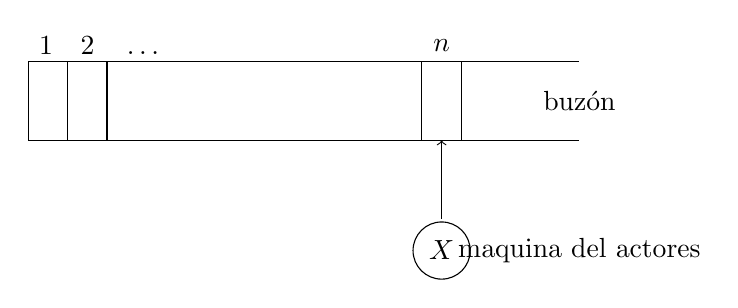
\begin{tikzpicture}

\draw (0,0) -- (7,0);
\draw (0,1) -- (7,1);

\draw (0,0) -- (0,1);
\draw (0.5,0) -- (0.5,1);
\draw (1,0) -- (1,1);

\draw (5,0) -- (5,1);
\draw (5.5,0) -- (5.5,1);

\node at (0.9,1.2) {$1\quad2\quad\ldots$};

\node at (5.25,1.2) {$n$};

\node at (7,0.5) {buzón};

\node at (7,-1.4) {maquina del actores};

\draw[->] (5.25,-1) -- (5.25,0);
\node at (5.25,-1.4) [circle,draw] (x) {$X$};

\end{tikzpicture}
\caption{Representación de un actor. La maquina del actor tiena la información de su comportamiento. Acepta la comunicación actual y no puede procesar ningún otra comunicación.}
\label{fig:mailqueue}
\end{figure}

Cuando la maquina del actores $X_n$ acepta la $(n)-esima$ comunicacion desde su buzón, crea la maquina del actor $X_{n+1}$ está ejecutará el comportamiento de reemplazo del actor. Esta nueva maquina apunta a la siguiente celda en el buzón en donde será guardada la comunicacion $(n+1)-esima$. Esto puede verse en la figura \ref{fig:actortransition}

\begin{figure}[H]
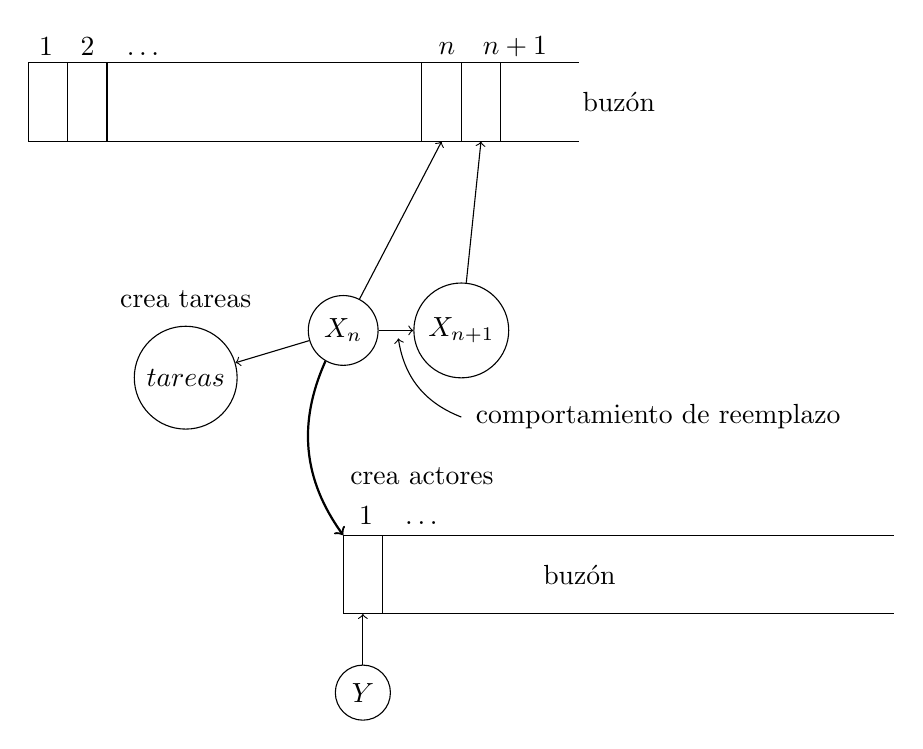
\begin{tikzpicture}

\draw (0,0) -- (7,0);
\draw (0,1) -- (7,1);

\draw (0,0) -- (0,1);
\draw (0.5,0) -- (0.5,1);
\draw (1,0) -- (1,1);

\draw (5,0) -- (5,1);
\draw (5.5,0) -- (5.5,1);
\draw (6,0) -- (6,1);

\node at (0.9,1.2) {$1\quad2\quad\ldots$};

\node at (5.9,1.2) {$n \quad n+1$};

\node at (4,-2.4) [circle,draw] (XN) {$X_n$};
\draw[->] (XN) -- (5.25,0);

\node at (5.5,-2.4) [circle,draw] (XN1) {$X_{n+1}$};
\draw[->] (XN1) -- (5.75,0);

\draw[->] (XN) -- (XN1);

\node at (2,-3) [circle,draw] (T) {$tareas$};

\draw (4,-5) -- (11,-5);
\draw (4,-6) -- (11,-6);
\draw (4,-5) -- (4,-6);
\draw (4.5,-5) -- (4.5,-6);

\draw[->, thick] (XN) to[bend right] (4, -5);


\node at (4.25,-7) [circle,draw] (Y) {$Y$};
\draw[->] (Y) -- (4.25, -6);
\node at (4.70, -4.75) {$1\quad\ldots$};

\draw[->] (XN) -- (T);

\node at (2,-2) {crea tareas};
\node at (5,-4.25) {crea actores};

\node at (8,-3.5) {comportamiento de reemplazo};

\draw[->] (5.5,-3.5) to[bend left] (4.7,-2.5); 

\node at (7.5,0.5) {buzón};
\node at (7,-5.5) {buzón};

\end{tikzpicture}
\caption{Una transición entre dos comportamientos}
\label{fig:actortransition}
\end{figure}


Las dos máquinas de actores $X_n$ y $X_{n+1}$ no interfieren entre sí. $X_n$ solo procesa la $(n)-esima$ comunicación, salvando el caso en el cual se envie una comunicación a si mismo. Cada una de estas maquinas crean sus propias tareas, sus propios actores como esta definido en sus comportamientos. Antes que la maquina $X_n$ cree la maquina $X_{n+1}$, $X_n$ podría haber creado otros actores u otras tareas. Es posible incluso, que $X_n$ este creando actores o tareas al mismo tiempo que lo está haciendo $X_{n+1}$. Es importante notar que $X_n$ no recibirá ninguna otra comunicacion, ni tampoco espeficiará ninguno otro comportamiento de reemplazo.

Si definimos que la creación de un actor, la creación de una tarea o especificar el comportamiento de reemplazo son eventos, el orden en que se generan estos eventos debido a que se acepto una comunicación define un orden parcial. El reemplazo de las máquinas del actor con cualquier direccione de buzón definen un orden total entre ellas. Esto se puede ver en la figura \ref{fig:actortransition}.

Una pregunta que surge a partir de crear una maquina de actores de reemplazo en cada vez que una comunicación es aceptada es, cuan performante esto resulta. Debería quedar claro que este modelo es solo conceptual y no está atado a una implementación en particular. La \textit{concurrencia} no implica paralelismo. Algunas implementación esperar a que la maquina de actores anterior termine, para construir la nueva y eliminar la vieja.

Sin embargo, retrasar el reemplazo de la construcción hasta que la máquina vieja pueda ser reemplazada no es un requisito como si lo sería en el caso de una máquina secuencial. Si hay suficientes recursos disponibles, la computación en un sistema de actores se puede acelerar, simplemente aceptando la próxima comunicación ni bien su comportamiento de reemplazo esta establecido.

% \begin{figure}[H]
% \begin{tikzpicture}
% 
% \node at (0,1) (A1) {Tareas pendientes};
% \node at (0,0) (A2) [circle,draw];
% \node at (0,-6) (A3) [circle,draw];
% \node at (0,-71) (A4) {x};
% 
% \node at (-1.5,-4) (Tx1) {a1};
% \node at (-3,-2) (Tx2) {destino};
% \node at (-3,2) (Tx3) {};
% 
% 
% \node at (1.5,-2) (Ax1) {a2};
% \node at (2,-1) (Ax2) {b2};
% 
% 
% \end{tikzpicture}
% \caption{xxx}
% \label{fig:taskprocesing}
% \end{figure}


\section{Programando con actores}

En esta sección se definiran las construcciones necesarias para definir un nucleo de un lenguaje minimo de actores. A pesar de su simplicidad, el este lenguaje es extremadamente poderoso, captura varias características importantes de la computación dentro del paradigma de actores: La posibilidad de ditribuir una computación entre elementos concurrentes, la únificación de información procedural y declarativa, y transparencia referencial de los identificadores usados en un programa.

\subsection{Las construcciones básicas}

En la configuración inicial de un sistema actores, necesitamos crear algunos actores y poderle enviar algunas comunicaciones. Un programa en un sistema de actores esta compuesto por:

\begin{itemize}
 \item \textit{definición de comportamientos} simplemente asocian un esquema de comportamiento con un identificador, no crear ningún actor.
 \item expresiones \textit{new} para crear nuevos actores.
 \item comandos \textit{send} para crear nuevas tareas.
\end{itemize}


\subsubsection*{Definiendo comportamientos}
Cada vez que un actor acepta una comunicación, define un comportamiento de reemplazo. Cada uno de los comportamientos de reemplazo también tendrá un comportamiento de reemplazo, para especificar el comportamiento de un actor, necesitamos una definición potencialmente infinita. Para esto acudimos al uso de la recursión. Básicamente, se parametriza cada comportamiento mediante algún identificador este será una variable libre en la definición. 

Por ejemplo, el comportamiento de una cuenta bancaria depende de su saldo. Entonces se especificará el comportamiento de la cuenta como una función de este saldo. Cada vez que se crea una cuenta, o se define un comportamiento de reemplazo, que usa la definición de comportamiento de una cuenta bancaria, se tiene que dar un valor especifico para esta cuenta.

También hay un número infinito de valores posibles para las comunicaiones entrantes. En este caso tambien se expresará como una funcion de la comunicación entrante.

Dos listas de identificadores son utilizadas en la definición de un comportamiento, La primer lista corresponde a los parámetros que son dados al momento de la creación de un actores. Esta lista es llamada \textit{acquaintance list}. La segunda lista, que se obtienen cuando una comunicación es aceptada, se llama \textit{communication list}. Cuando un actor es creado y acepta una comunicación ejecuta los comandos en el \textit{entorno} definido por los parametros enlazados a los identificares.

\subsubsection*{Creando Actores}

\subsubsection*{Creando tareas}

\subsubsection*{Comandos}

\subsubsection*{Comportamiento por defecto}




